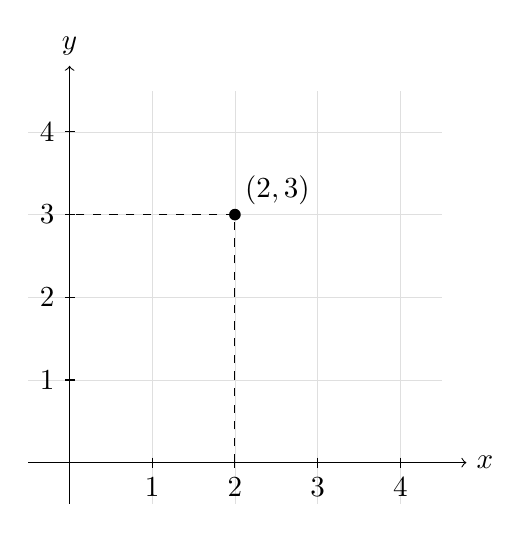
\begin{tikzpicture}[scale=1.05, transform shape]
    \draw[step=1, gray!25, very thin] (-0.5,-0.5) grid (4.5,4.5);
    \draw[->] (-0.5,0) -- (4.8,0) node[right] {$x$};
    \draw[->] (0,-0.5) -- (0,4.8) node[above] {$y$};
    \foreach \x in {1,2,3,4} {
        \draw (\x,0.06) -- (\x,-0.06) node[below] {\x};
    }
    \foreach \y in {1,2,3,4} {
        \draw (0.06,\y) -- (-0.06,\y) node[left] {\y};
    }
    \draw[dashed] (2,0) -- (2,3) -- (0,3);
    \fill (2,3) circle (2pt);
    \node[above right] at (2,3) {$(2,3)$};
\end{tikzpicture}
